% Please use LuaLaTex to compile this file.

\documentclass[11pt]{article}

\usepackage{subfigure}
\usepackage{xltxtra, url, parskip} 	% Other packages for formatting
\RequirePackage{color, graphicx}
\usepackage{hyperref}
\usepackage{mathtools}
\usepackage{amsmath}
\usepackage[symbol]{footmisc}
\usepackage{luatexja-fontspec}
\setmainjfont{SimSun}
\usepackage{booktabs} % Table rules.
\usepackage{multirow} % Multi Table

% Set footnote counter.
\renewcommand*{\thefootnote}{\fnsymbol{footnote}}
\setcounter{footnote}{1}

\renewcommand\figurename{图}

% Set link color.
%\definecolor{linkcolour}{rgb}{0, 0.2, 0.6}
%\hypersetup{colorlinks, breaklinks, urlcolor=linkcolour, linkcolor=linkcolour}

\title{车道跟随算法设计文档}

\author{万年杰}

\begin{document}

\maketitle
\newpage

\section{概览}
此文档旨在对即将实现的基于Raspberry Pi的车道跟随算法进行一个简要的介绍。第一部分是对整个项目的概览,包括对背景的介绍以及对算法流程的整体认识。第二部分详细介绍了一些实现过程中可能设计到的一些技术难题以及相应的解决方案。

\subsection{背景介绍}
车道检测是车道侧偏检测的前提, 是车辆辅助驾驶系统的重要组成部分, 也是自动驾驶算法研究的一个重要方向。本项目通过实践对这一领域进行初步探索。为了简化问题,本项目只考虑了白天情况下车道为平行直线的情况,针对更复杂路况的算法将在之后逐步迭代。

\subsection{算法流程}
我采用了设置感兴趣区域 (ROI)的方式来简化计算,通常情况下取图像下部的$\frac{1}{4}$到$\frac{1}{3}$进行处理。之后我对其进行了灰度化以及高斯模糊以去除图像中的部分噪声。Sobel边缘检测以及其他的去噪手段也在这一阶段得到使用,最后我对获取到的主要边缘进行Hough变换,提取出其中的直线信息,将其认为是车道。

由于本项目只拥有一个摄像头作为传感器,在将图像信息映射到实际的物理空间信息时,视角变幻算法显得尤为重要,此过程也将产生PID反馈控制系统的主要输入(偏差角$\theta$)。

PID闭环控制系统将综合之前图像处理产生的信息与小车当前的壮态,从而对车辆进行合理的调控,保证车辆的正常行驶。

整个算法流程如图~\ref{fig:flow-chart}所示。

\begin{figure}[h!]
	\centering
	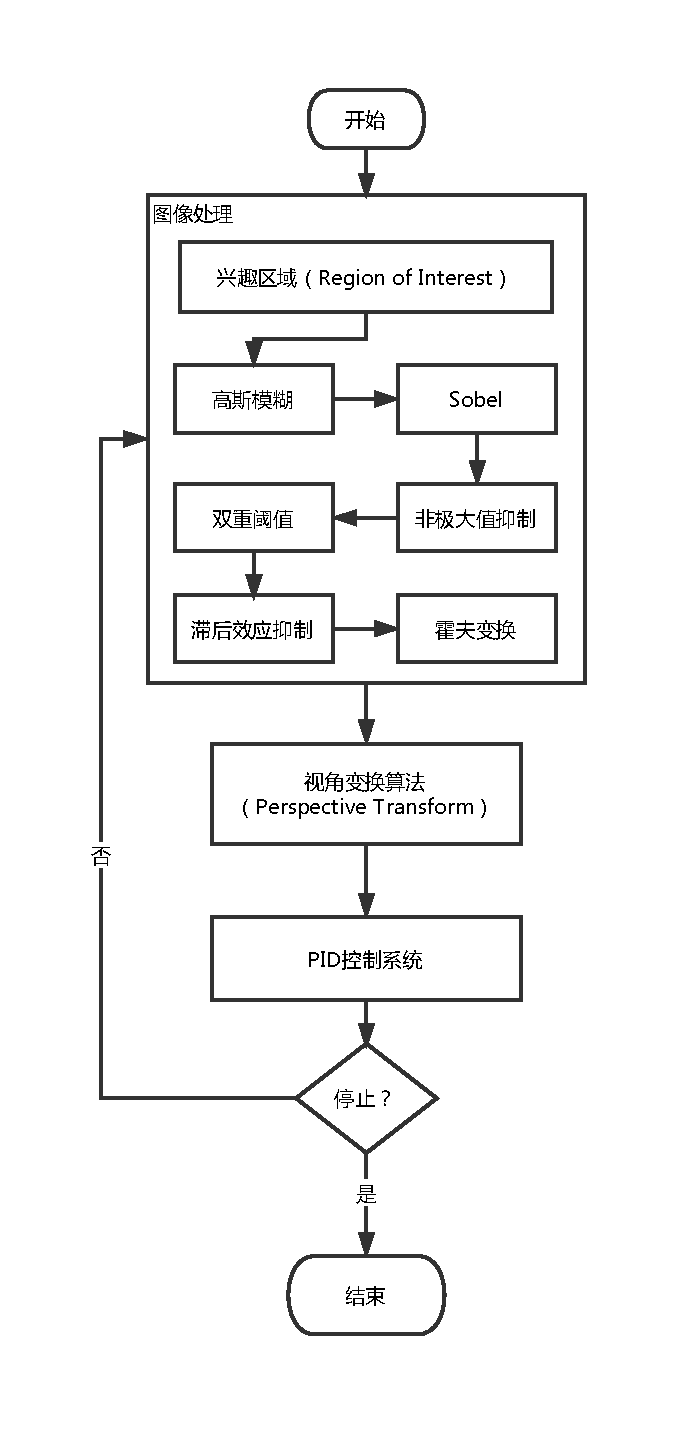
\includegraphics[width=8cm]{Graphs/flow-chart}
	\caption{算法流程图}
	\label{fig:flow-chart}
\end{figure}

\section{实现细节}

\subsection{图像处理}
在进行了ROI处理后,将RGB图像转化为灰度图像,紧接着对其进行了Canny边缘检测的一般过程,Hough变幻等,这些技术都已经相当成熟,在此不再赘述。

\subsection{视角变换算法}
视角变换算法结果的有效性依赖于很多方面,但最主要的是如下两个方面:

\begin{enumerate}
  \item[(1)] 摄像头必须被妥善地安装在小车上(最好是正中间),且摄像头的是固定的(不会出现角度突变的情况)。
  \item[(2)] 光线足够,摄像头拍出的图像可以区分出车道和地面。
\end{enumerate}

我们按照如图~\ref{fig:coordinate-system}为摄像头及车道建立直角坐标系。

\begin{figure}[h!]
	\centering
	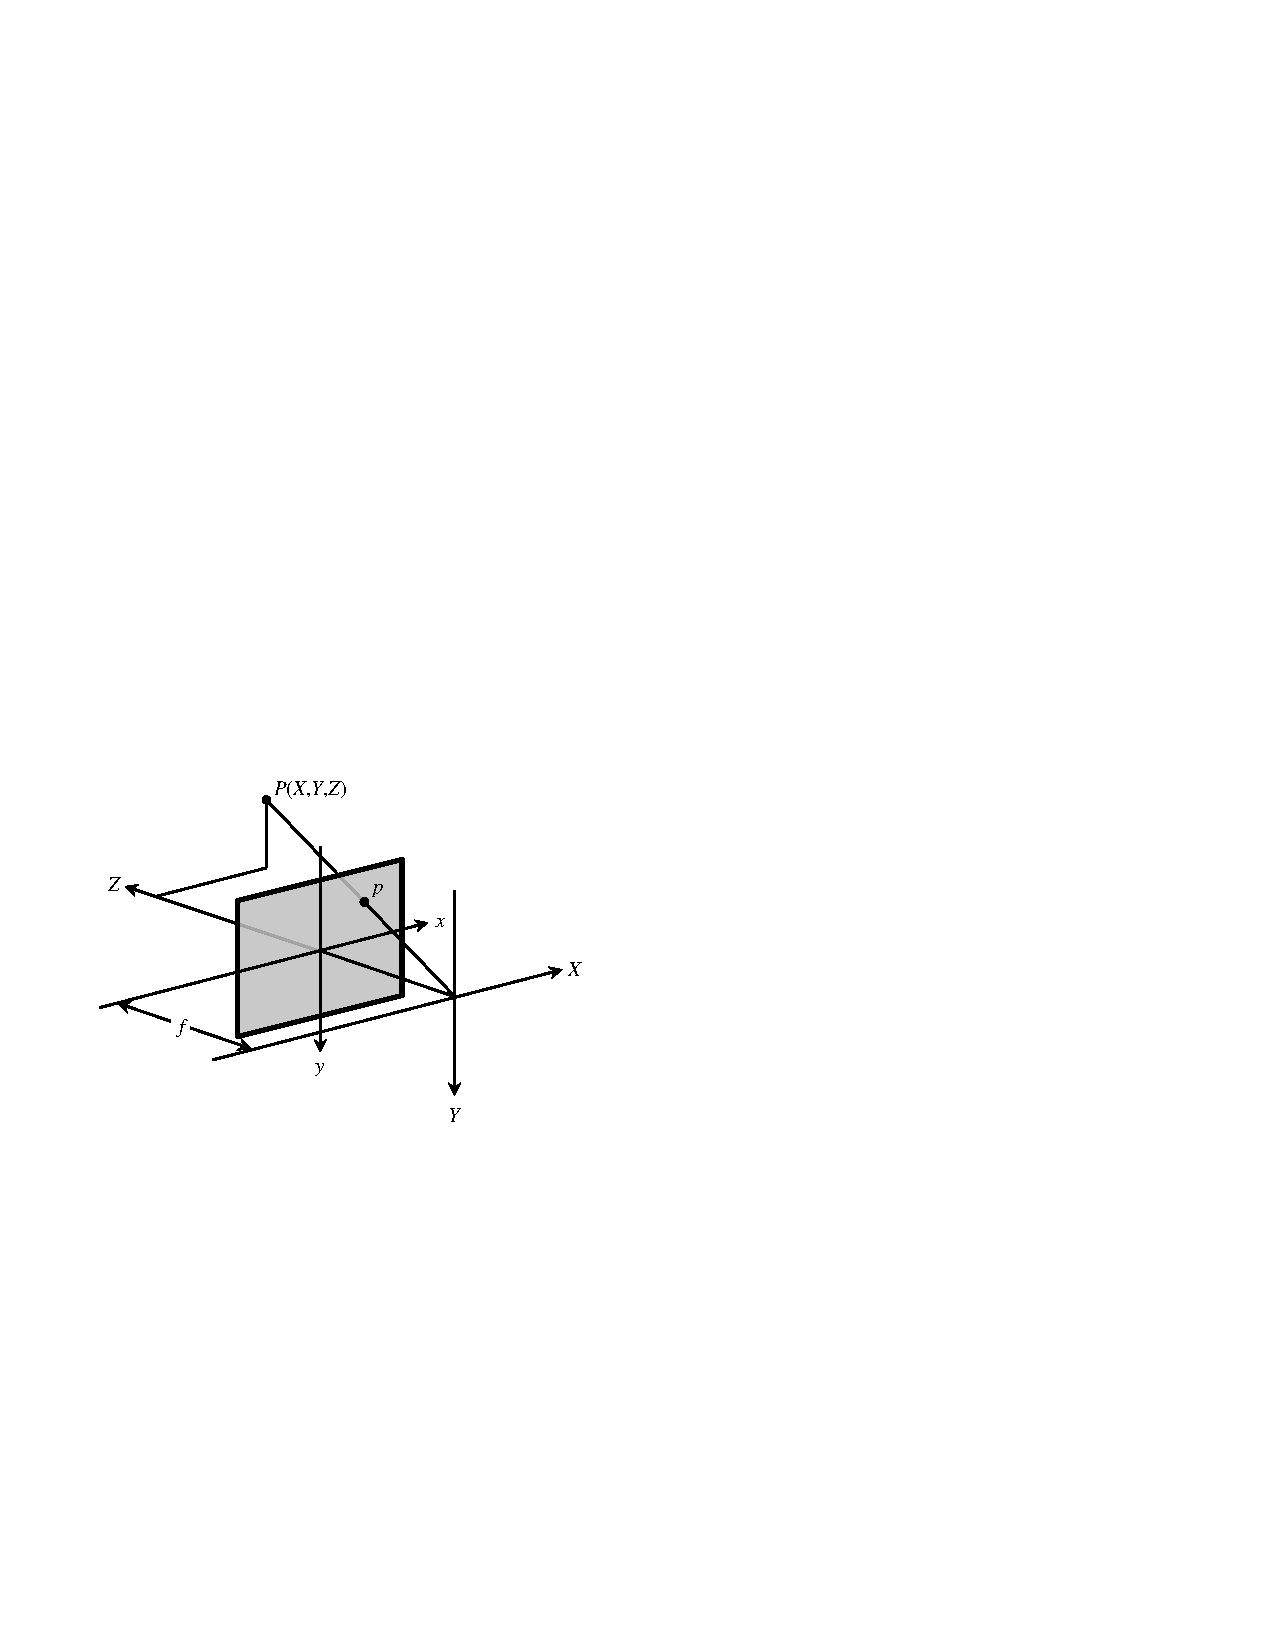
\includegraphics[width=8cm]{Graphs/coordinate-system}
	\caption{坐标系}
	\label{fig:coordinate-system}
\end{figure}

其中,摄像头被放置在$XYZ$坐标系的原点处,焦距为$f$,$xy$平面是摄像头的成像平面,地面是$Y=H$平面,$H$是摄像头距离地面的高度。

在实际物理空间中的一点$P(X,Y,Z)$映射到照片($xy$平面)中的坐标即为:

$$
\begin{cases}
  x = f \frac{X}{Z} \\
  y = f \frac{Y}{Z}
\end{cases}
$$

针对$Y=H$的$(X, H, Z)$,则有:

$$
\begin{cases}
  X = H\frac{x}{y} \\
  Z = H\frac{f}{y}
\end{cases}
$$

假设一条车道在平面$XZ$中的方程为$Z = MX + B$,如图~\ref{fig:lane}所示。

\begin{figure}[h!]
	\centering
	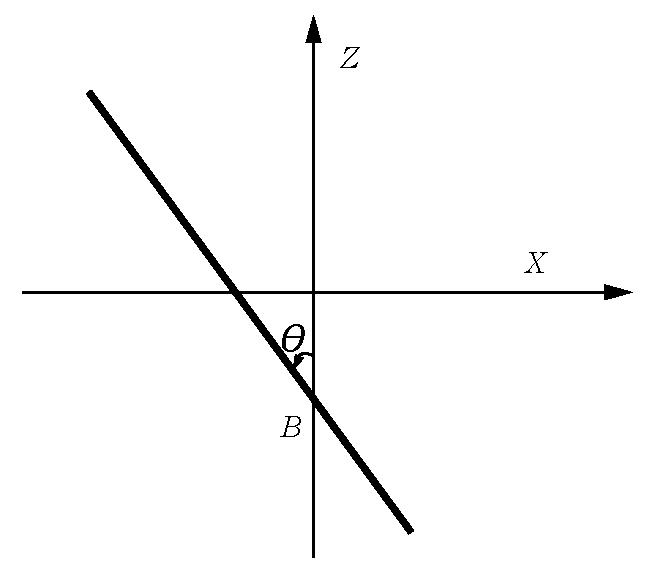
\includegraphics[width=8cm]{Graphs/lane}
	\caption{车道}
	\label{fig:lane}
\end{figure}

则$\theta$角代表的即是此时小车的偏移角(从$Z$轴到该直线的角)。而车道在照片平面中的方程即为:

$$
y = -\frac{HM}{B}x + \frac{Hf}{B} = mx + b
$$

我们称斜率为负的角度为负,斜率为正的角度为正,$m, b$均可从照片中得到。

进而,我们可以计算得:

$$
\theta = -arctan\frac{b}{mf}
$$

现在将情况扩展为两条平行的车道,则:

$$
\begin{cases}
Z = MX + B_1 \\
Z = MX + B_2
\end{cases}
$$

我们希望小车尽可能地在两车道的中心行驶,因此我们需要另一个参数$\Delta d$来表示当前小车的水平偏移量,有:

$$
\Delta d = (B_1 + B_2) \vert tan\theta \vert
$$

经过类似的坐标转换后,我们可得:

$$
\Delta d = (\frac{Hf}{b_1} + \frac{Hf}{b_2})\vert tan\theta \vert
$$

此后再经过从像素点到实际物理长度的映射过程,即可得到对应的水平偏移量$\Delta D$。

\subsection{PID控制算法}

从上面一节中,我们已经计算得到两个最重要的参数:偏移角$\theta$和水平偏移量$\Delta D$,这两个参数将作为PID控制系统的输入。

此PID系统的目标相对来说比较简单,即控制$\theta$和$\Delta D$均为0。

\subsubsection{角度控制}

经计算可得,在理想情况下,小车的角速度为:

$$
\omega = \frac{V_L - V_R}{L}
$$

其中,$V_L$是左后车轮速度,$V_R$是右后车轮速度,$L$是两车轮间距。设小车偏移角随时间的变化函数为$\theta(t)$,则有:

$$
\theta(t) = \theta_0 + \omega t
$$

我们首先采用简单的P控制器,及我们对小车角速度的控制与误差$\epsilon$成正比,设比例系数为$K$,则有:

$$
\begin{cases}
\epsilon = \theta(t) - \phi \\
\omega = K\epsilon
\end{cases}
$$

其中,$\phi$是我们希望的偏移角,在这里,$\phi = 0$,则有:

$$
\omega = K \theta(t)
$$

系数$K$的单位是$/s$,则有:

$$
\theta(t) = \frac{\theta_0}{1 - Kt}
$$

可知,$K$越大,$\theta$收敛得越快。

\subsubsection{水平偏移量控制}

未能来得及实现,但总体思路是需要与角度控制结合写出PID的表达式。


% Bibliography
\begin{thebibliography}{99}

\bibitem{coordinate-system} McFall, K., \& Tran, D. (2014, November). Visual lane detection algorithm using the perspective transform. In Proceedings of the 14th Early Career Technical Conference (Vol. 13).

\bibitem{lane-detection} McFall, K. (2016). Using Visual Lane Detection to Control Steering in a Self-Driving Vehicle. In Smart City 360° (pp. 861-873). Springer, Cham.

\bibitem{comparative-study} Romdhane, N. B., Hammami, M., \& Ben-Abdallah, H. (2011, August). A comparative study of vision-based lane detection methods. In International Conference on Advanced Concepts for Intelligent Vision Systems (pp. 46-57). Springer, Berlin, Heidelberg.

\bibitem{embedded-system} Lee, E. A., \& Seshia, S. A. (2016). Introduction to embedded systems: A cyber-physical systems approach. MIT Press.

\bibitem{system-signal} Lee, E. A. (2011). Structure and interpretation of signals and systems. Lee \& Seshia. 

\end{thebibliography}

\end{document}